\documentclass{report}
\usepackage[showframe=false]{geometry}
\usepackage{titlesec}
\usepackage{amsmath}
\usepackage{graphicx}

\pagenumbering{gobble}

\geometry{tmargin=60pt,bmargin=90pt,lmargin=90pt,
rmargin=90pt}

\titleformat{\chapter}{\normalfont\huge}{\thechapter.}{20pt}{\huge}
\titlespacing*{\chapter} {0pt}{0pt}{10pt}

\begin{document}

\chapter{Section 1}
\section{a.}

The vertebral column data was first read from the ARFF file, then split into classes for processing.

\begin{verbatim}
  library(foreign)
  vert <- read.arff("column_2C_weka.arff")
  vert_split <- split(vert, vert[,"class"])

  sapply(vert_split$Abnormal[0:6], mean)
  sapply(vert_split$Abnormal[0:6], median)
  sapply(vert_split$Abnormal[0:6], sd)
  sapply(vert_split$Normal[0:6], mean)
  sapply(vert_split$Normal[0:6], median)
  sapply(vert_split$Normal[0:6], sd)
\end{verbatim}

\subsection{Abnormal Data}

\begin{tabular}{l}
  mean \\
  \hskip 1.0cm\begin{tabular}{rrr}
    pelvic\_incidence & pelvic\_tilt & lumbar\_lordosis\_angle \\
    64.69256 & 19.79111 & 55.92537 \\
    sacral\_slope & pelvic\_radius & degree\_spondylolisthesis \\
    44.90145 & 115.07771 & 37.77771 \\
  \end{tabular} \\
  standard deviation \\
  \hskip 1.0cm\begin{tabular}{rrr}
    pelvic\_incidence & pelvic\_tilt & lumbar\_lordosis\_angle \\
    65.27489 & 18.79890 & 56.15000 \\
    sacral\_slope & pelvic\_radius & degree\_spondylolisthesis \\
    44.63960 & 115.65032 & 31.94652 \\
  \end{tabular} \\
  median \\
  \hskip 1.0cm\begin{tabular}{rrr}
    pelvic\_incidence & pelvic\_tilt & lumbar\_lordosis\_angle \\
    17.66213 & 10.51587 & 19.66947 \\
    sacral\_slope & pelvic\_radius & degree\_spondylolisthesis \\
    14.51556 & 14.09060 & 40.69674 \\
  \end{tabular}
\end{tabular}

\subsection{Normal Data}

\begin{tabular}{l}
  mean \\
  \hskip 1.0cm\begin{tabular}{rrr}
    pelvic\_incidence & pelvic\_tilt & lumbar\_lordosis\_angle \\
    51.685244 & 12.821414 & 43.542605 \\
    sacral\_slope & pelvic\_radius & degree\_spondylolisthesis \\
    38.863830 & 123.890834 & 2.186572 \\
  \end{tabular} \\
  standard deviation \\
  \hskip 1.0cm\begin{tabular}{rrr}
    pelvic\_incidence & pelvic\_tilt & lumbar\_lordosis\_angle \\
    50.12312 & 13.48243 & 42.63892 \\
    sacral\_slope & pelvic\_radius & degree\_spondylolisthesis \\
    37.05969 & 123.87433 & 1.15271 \\
  \end{tabular} \\
  median \\
  \hskip 1.0cm\begin{tabular}{rrr}
    pelvic\_incidence & pelvic\_tilt & lumbar\_lordosis\_angle \\
    12.368161 & 6.778503 & 12.361388 \\
    sacral\_slope & pelvic\_radius & degree\_spondylolisthesis \\
    9.624004 & 9.014246 & 6.307483 \\
  \end{tabular}
\end{tabular}

\section{b.}

\begin{verbatim}
  library(foreign)
  vert <- read.arff("column_2C_weka.arff")

  pairs(vert[0:6], pch = 21, bg = c(``green'', ``blue'')[unclass(vert$class)])
\end{verbatim}

\begin{figure}[h!]
  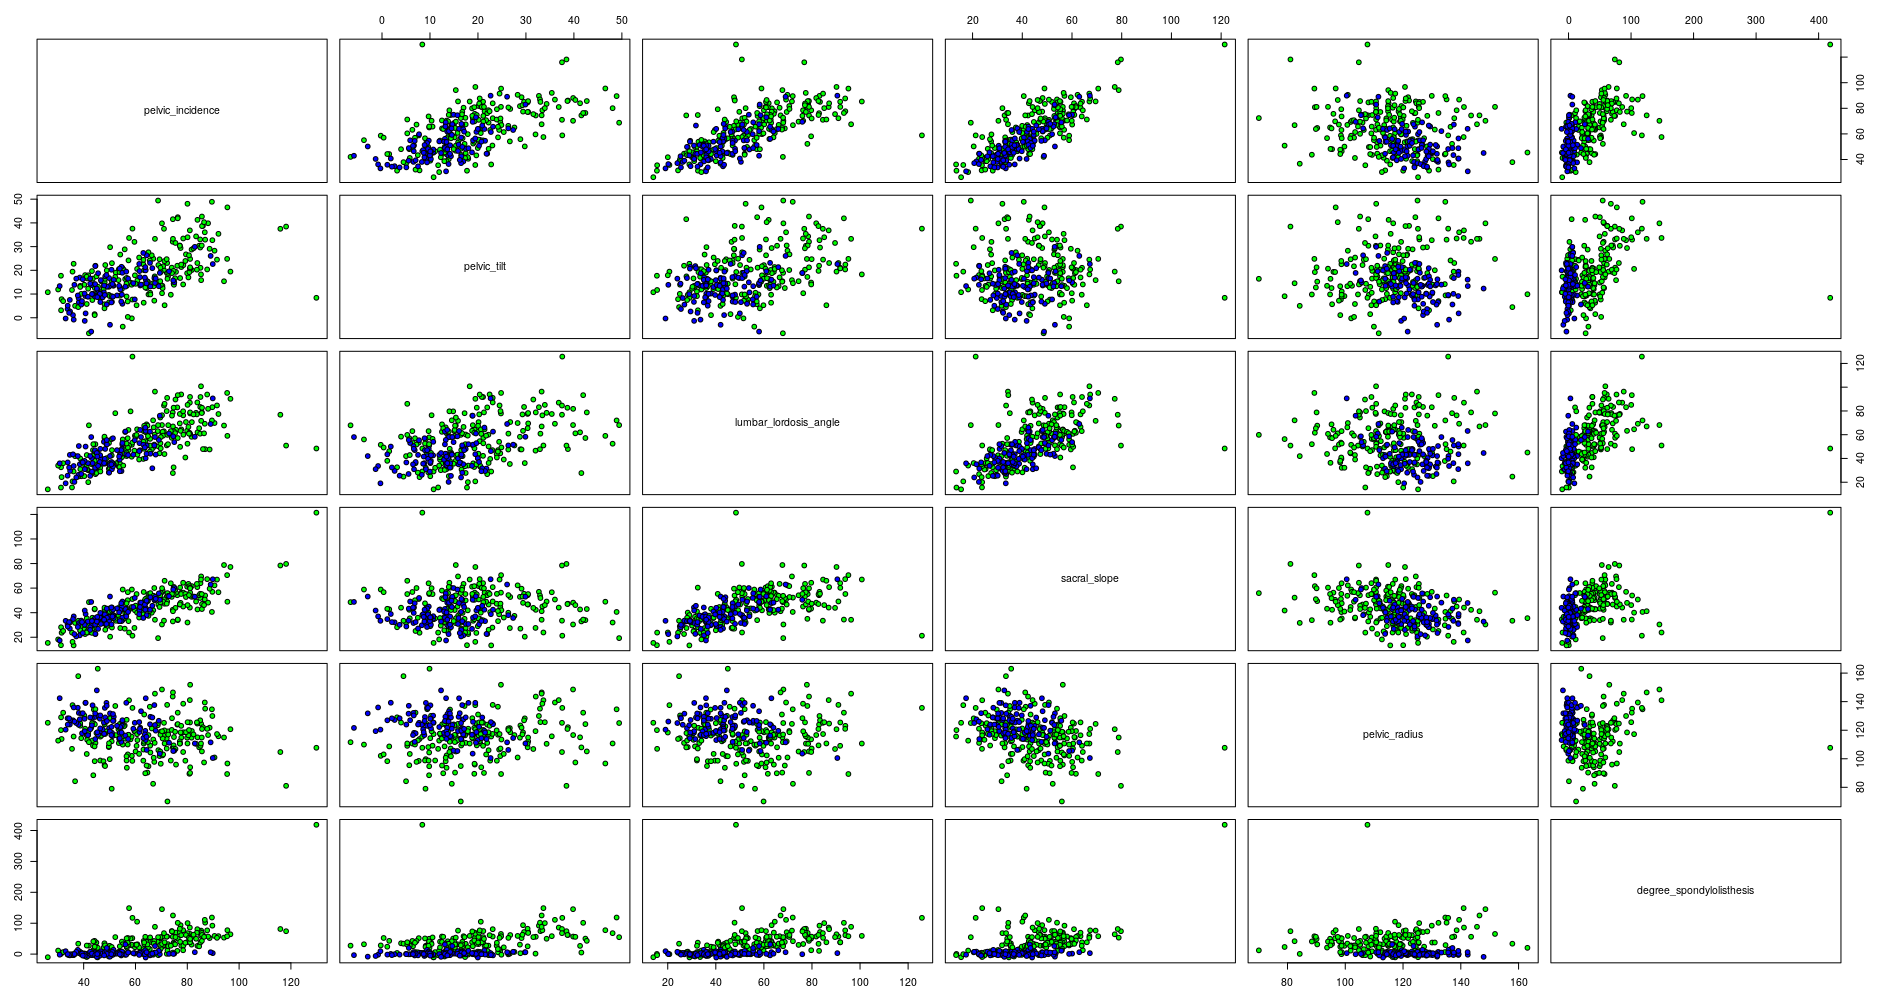
\includegraphics[width=\linewidth]{FeatureScatterPlot.png}
  \caption{Feature Scatter Plot}
  \label{fig:FeatureScatterPlot}
\end{figure}

\section{c.}

Given the values from section a and the scatter plot from section b we can see that the two classes are seperatated well by there values. For example if we pick two classes, pelvic\_radius and degree\_spondylolisthesis, we can compare the values and see how well they are seperated. If we also take into account the scatter plot from Figure \ref{fig:FeatureScatterPlot} we can see that abnormal classes have a larger value with respect of degree\_spondylolisthesis then the normal class.

\chapter{Section 2}

\section{a.}

Generating 100 3-dimensional vectors from a normal disribution with a mean vector as [1 2 1] and a 3x3 covariance matrix as [4  0.8 -0.3; 0.8 2 0.6; -0.3 0.6 5]

\begin{verbatim}
  mean <- c(1,2,1)
  cov <- matrix(c(4, 0.8, -0.3, 0.8, 2, 0.6, -0.3, 0.6, 5), 3,3)
  mvnd <- MASS\dotsmvrnorm(n = 100, mean, cov)
\end{verbatim}

\[
  mean=
  \begin{bmatrix}
    1 & 2 & 1
  \end{bmatrix}
\]

\[
  cov=
  \begin{bmatrix}
    4 & 0.8 & -0.3 \\
    0.8 & 2 & 0.6 \\
    -0.3 & 0.6 & 5
  \end{bmatrix}
\]

\section{b.}

\section{c.}

\chapter{Section 3}

\begin{verbatim}
	records <- read.table("five-dimensional-records.txt")
  mean <- colMeans(records)
	cov <- cov(records)
\end{verbatim}

\[
  mean <- 
  \begin{bmatrix}
    6241.66667 & 11.44167 & 2333.33333 & 120.83333 & 17000.00000
  \end{bmatrix}
\]

\[
  cov <- 
  \begin{bmatrix}
	1.183356e+07 & 59.924242 & 4152121.2121 & 173507.5758 & 490909.091 \\
	5.992424e+01 & 3.191742 & 342.1212 & 141.9621 & 9818.182 \\
	4.152121e+06 & 342.121212 & 1540606.0606 & 73424.2424 & 963636.364 \\
	1.735076e+05 & 141.962121 & 73424.2424 & 13208.3333 & 569090.909 \\
	4.909091e+05 & 9818.181818 & 963636.3636 & 569090.9091 & 40545454.545
  \end{bmatrix}
\]

\begin{verbatim}
  Eigenvalues <- eigen(cov)$values
  Eigenvectors <- eigen(cov)$vectors
\end{verbatim}

\[
  Eigenvalues <- 
  \begin{bmatrix}
	  4.058981e+07 & 1.327940e+07 & 6.078551e+04 & 2.835137e+03 & 5.672175e-01
  \end{bmatrix} \\
\]

\[
  Eigenvectors <- 
  \begin{bmatrix}
    0.0210326211 & 9.430084e-01 & 0.332053840 & 0.0057119337 & -0.0006728422 \\
    0.0002420299 & -8.480421e-06 & -0.002006136 & -0.0006633593 & -0.9999977384 \\
    0.0269236336 & 3.312548e-01 & -0.942852072 & 0.0239126004 & 0.0018793378 \\
    0.0141541619 & 1.292481e-02 & -0.020405538 & -0.9996077844 & 0.0007073532 \\
    0.9993159400 & -2.895527e-02 & 0.018703144 & 0.0133939822 & 0.0001957042
  \end{bmatrix}
\]

\begin{figure}[h!]
	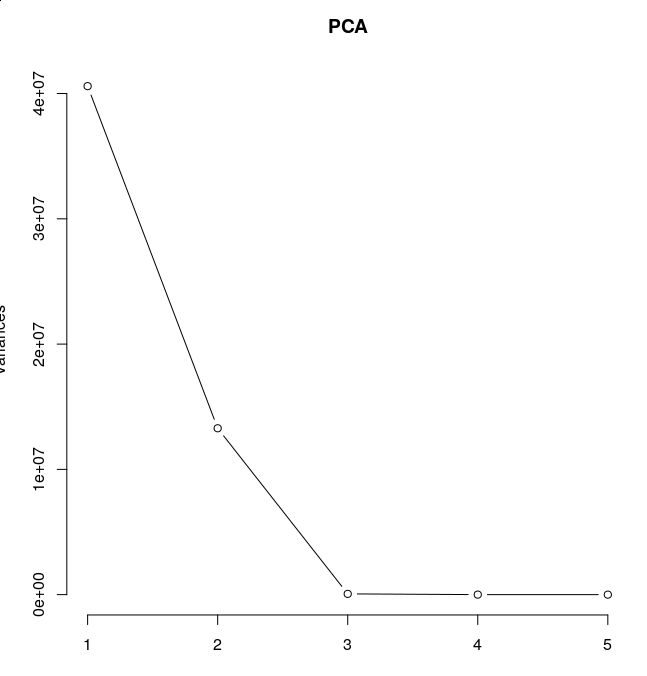
\includegraphics[width=\linewidth]{eigenvectors graph.png}
	 \caption{Eigenvectors line graph}
	\label{fig:eigenvectorslinegraph}
\end{figure}

\begin{verbatim}	
  PCA <- as.data.frame(prcomp(records)$x)[1:2]
\end{verbatim}

\[
  PCA <- 
  \begin{bmatrix}
    7989.734 & -685.3013 \\
    -7153.694 & -5315.8562 \\
    -8091.763 & -2891.1789 \\
    7926.393 & -2743.7012 \\
    7927.907 & -2588.2250 \\
    -4949.073 & 2079.0494 \\
    -1158.977 & -5367.2371 \\
    -2912.664 & 3101.7248 \\
    1105.817 & 3774.9869 \\
    8103.076 & 3358.3627 \\
    -4900.497 & 3631.3980 \\
    -3886.258 & 3645.9779
  \end{bmatrix}
\]

\begin{figure}[h!]
	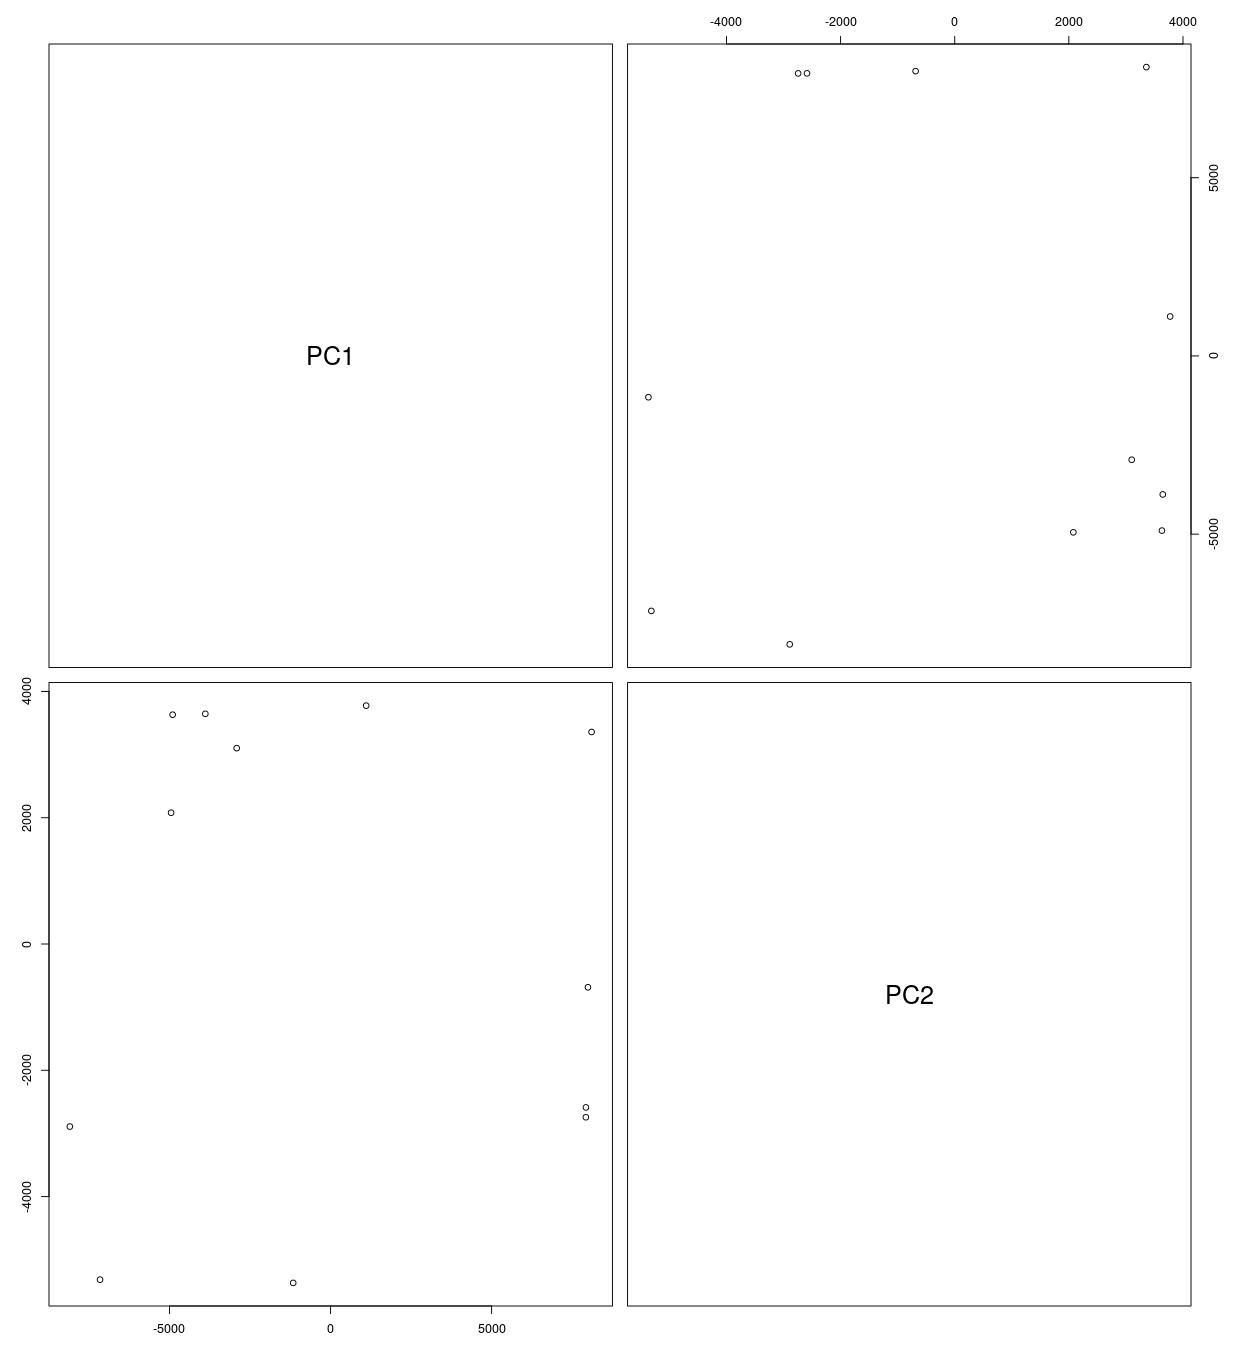
\includegraphics[width=\linewidth]{pca_scatter_plot.png}
	 \caption{PCA Scatter Plot}
	\label{fig:PCA Scatter Plot}
\end{figure}

\chapter{Section 4}

\begin{verbatim}	
  PCA <- prcomp(vert[0:6])
  Eigenvalues <- PCA$sdev^2
  Eigenvectors <- PCA$rotation
  reduced <- as.data.frame(PCA$x)[1:2]
  pairs(reduced, pch = 21, bg = c('green', 'blue')[unclass(vert$class)])
\end{verbatim}

\[
  Eigenvalues <- 
  \begin{bmatrix}
    1.780994e+03 & 3.453271e+02 & 1.887770e+02 & 1.060179e+02 & 8.861407e+01 & 7.207841e-18
  \end{bmatrix}
\]

\[
  Eigenvectors <- 
  \begin{bmatrix}
    -0.32364565 & 0.47663485 & -0.001544813 & 0.37367725 & -0.44170387 & -5.773503e-01 \\
    -0.11319229 & 0.09856328 & -0.264657410 & 0.75411376 & 0.07354147  & 5.773503e-01 \\
    -0.30367474 & 0.53278398 & -0.496541893 & -0.33941176 & 0.51202411 & 1.089295e-11 \\
    -0.21045336 & 0.37807157 & 0.263112598 & -0.38043651 & -0.51524534 & 5.773503e-01 \\
    0.02995983 & -0.32180920 & -0.774612852 & -0.17510604 & -0.51463973 & 3.590517e-12 \\
    -0.86315378 & -0.48243804 & 0.118940778 & -0.03291431 & 0.08359925 & -3.067324e-12
  \end{bmatrix}
\]

\begin{figure}[h!]
  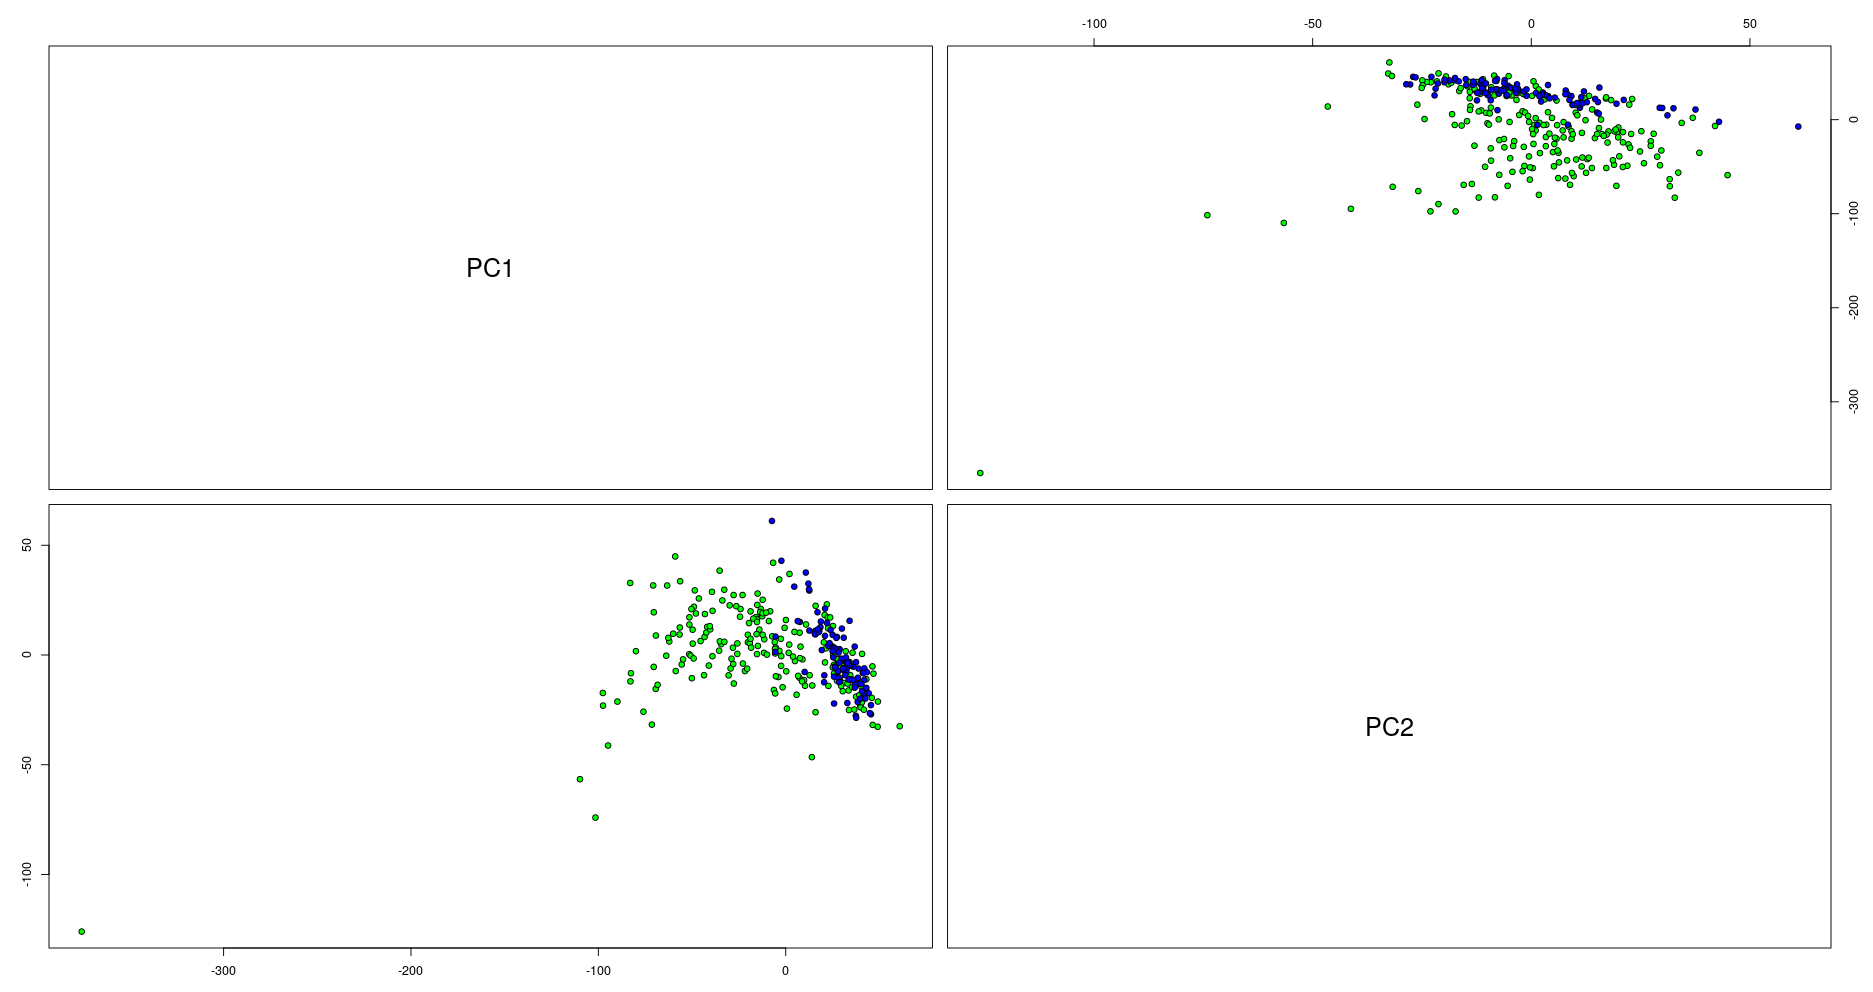
\includegraphics[width=\linewidth]{pca_vertebral_column_data_set.png}
  \caption{PCA Vertebral Column Data Set}
  \label{fig:PCAVertebralColumnDataSetScatterPlot}
\end{figure}

\chapter{Section 5}

\end{document}







































